\chapter*{Management Summary}

\section*{Scoreboard}
In a Coiffeur Jass match there are a lot of things to keep track of:

\begin{itemize}
    \item Round scores
    \item Multipliers
    \item Total Scores
    \item Who gets to choose the next contract
\end{itemize}

All of this is difficult to track in your head. So traditionally a chalkboard is used to track what has been played. JassTracker aims to be a web based replacement for the classic chalkboard and more. With JassTracker you only need to enter the score of each round and our dynamic scoreboard takes care of the rest. The scoreboard also highlights who gets to choose the contract for the next round, so you will never have to count the rounds in your head again.

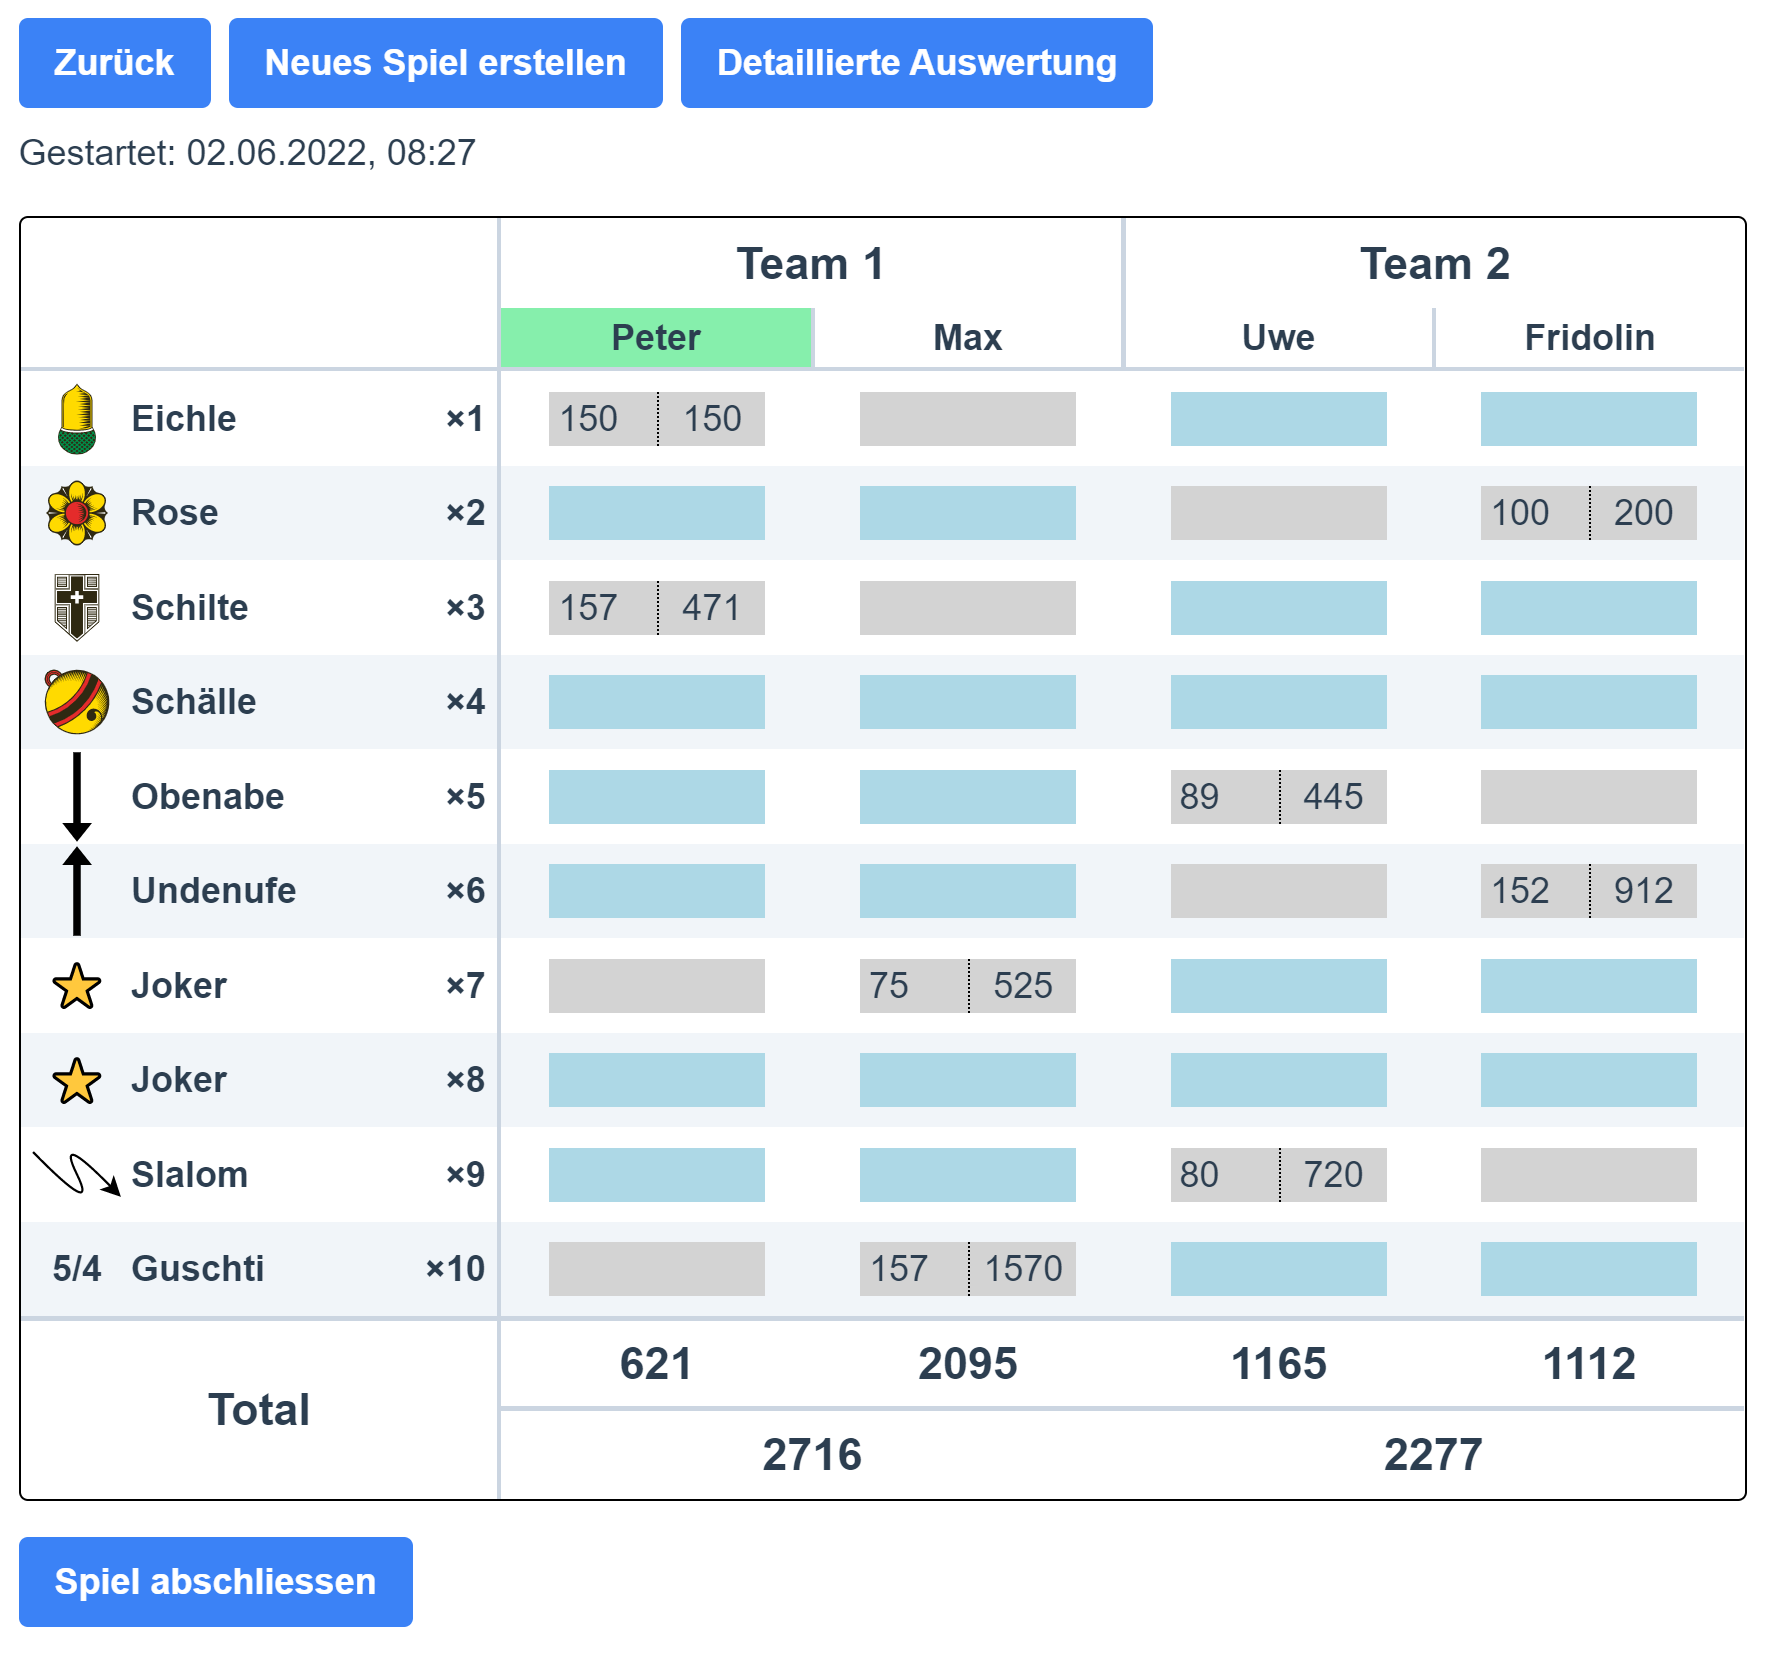
\includegraphics[height=0.4\textheight]{resources/screenshots/scoreboard}

\section*{Tables}
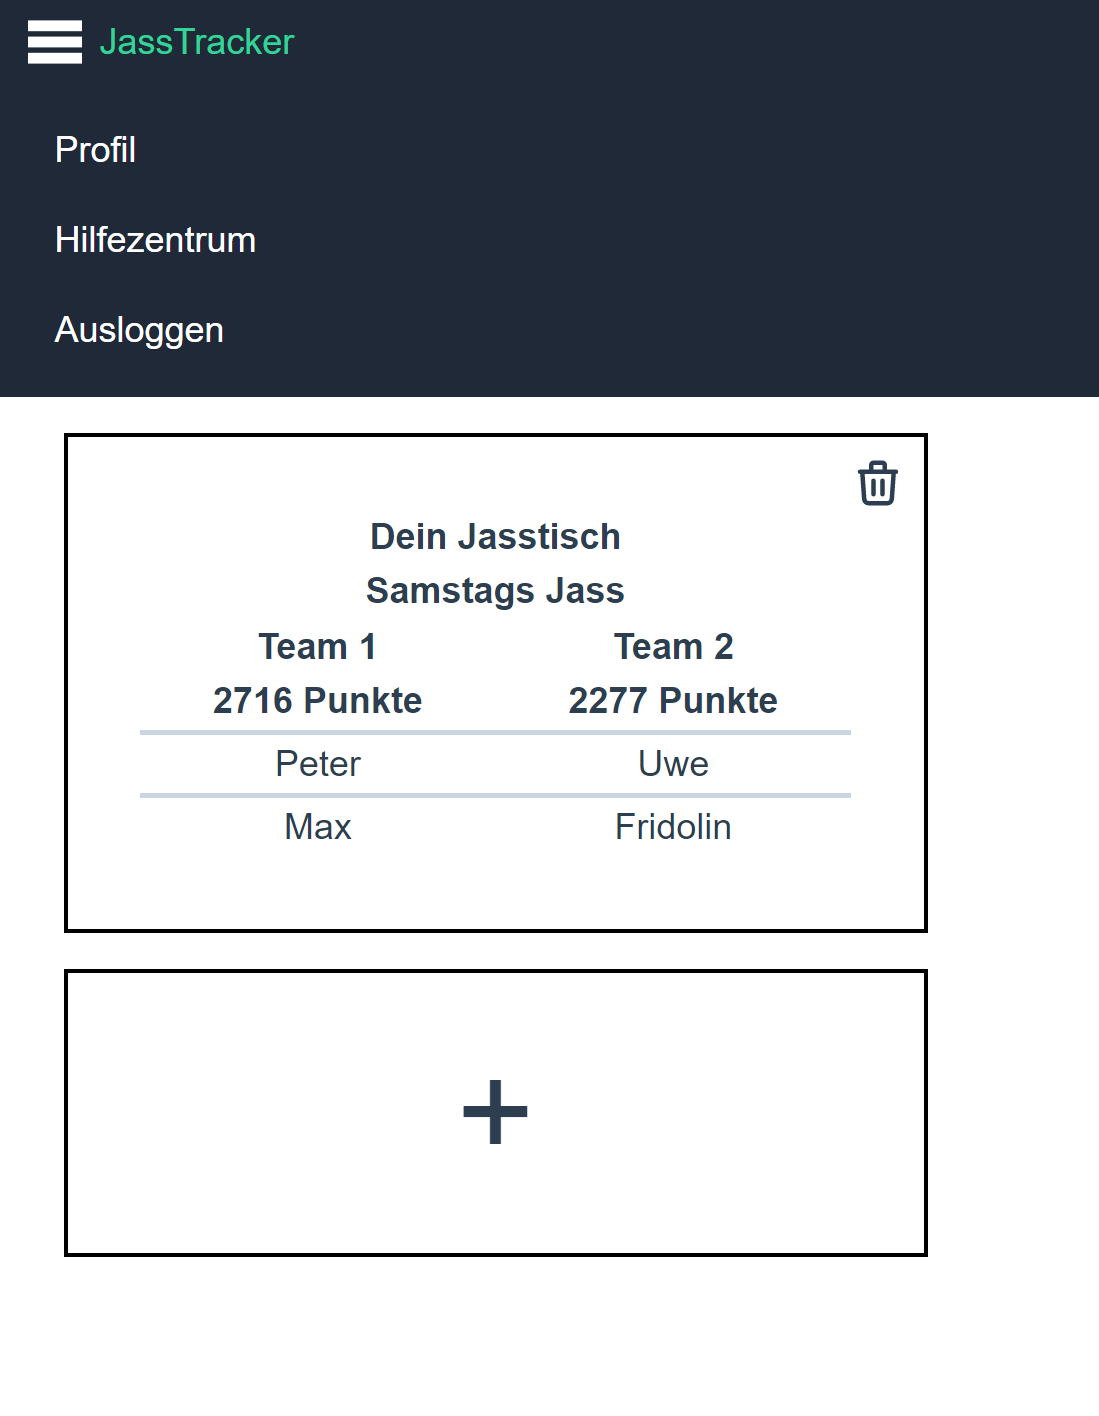
\includegraphics[height=0.5\textheight]{resources/screenshots/tables}

If there are multiple groups of people you play Jass with such as your family or a group of friends, it would be nice to separate the matches. For this we introduce the concept of a Jass table, which gives you the ability to group your Jass matches. The table creation dialog allows adding players to the table and the ability to play around with different team constellations.

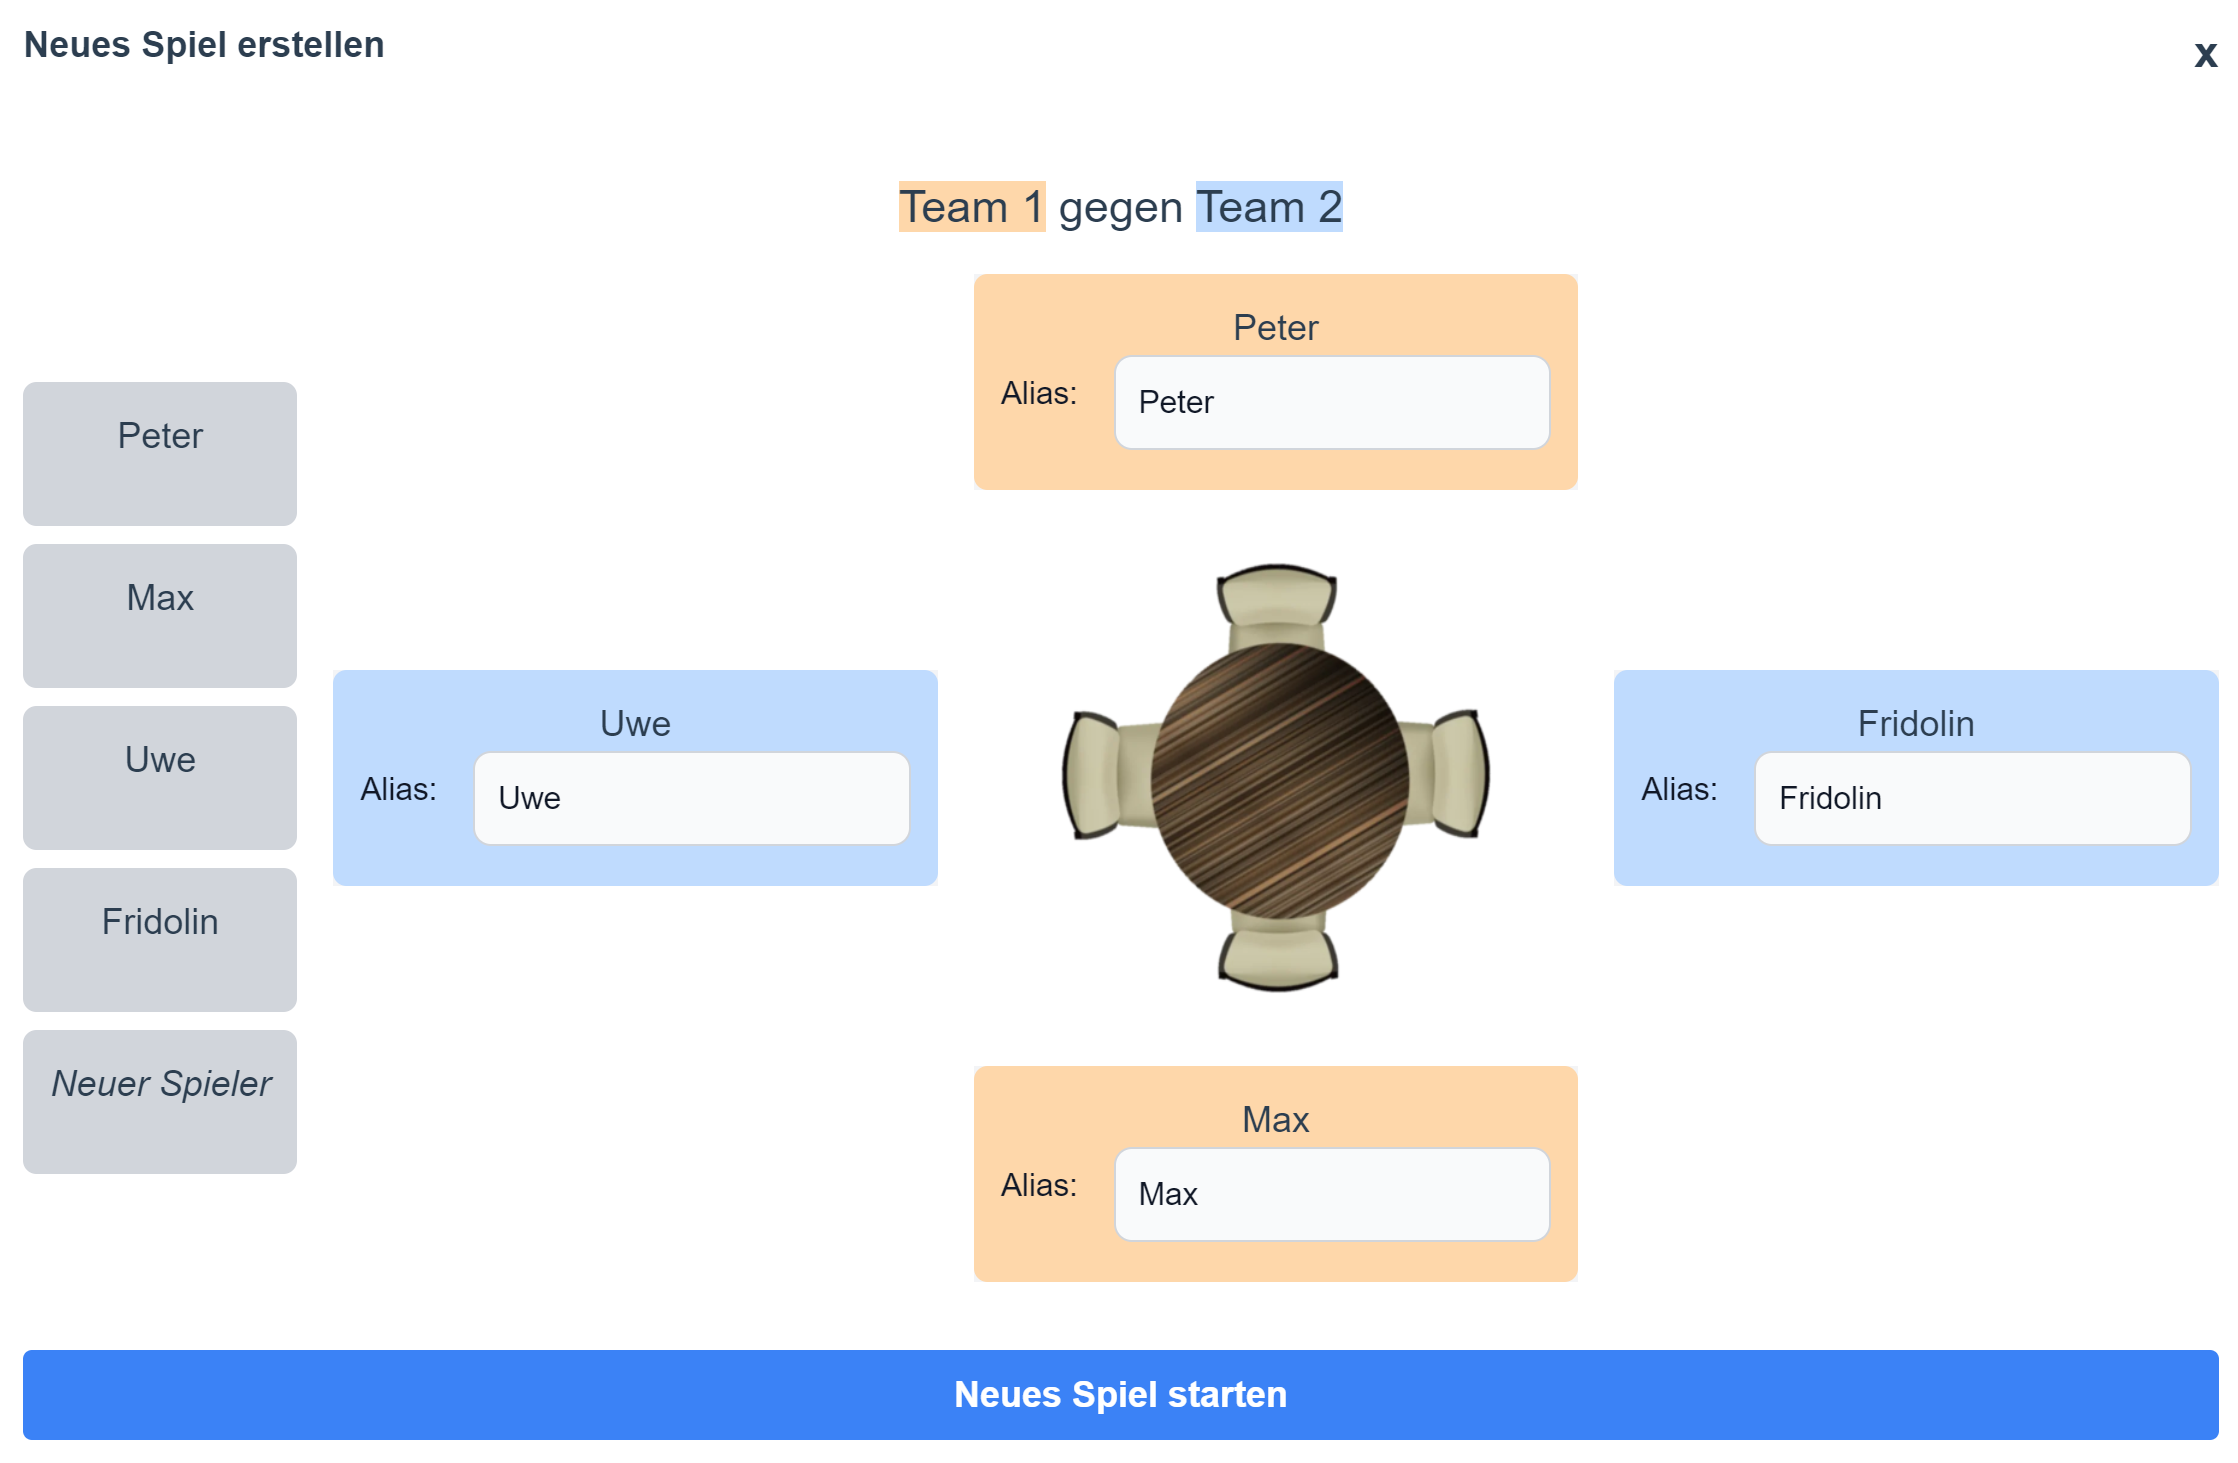
\includegraphics[width=0.9\textwidth]{resources/screenshots/table-creation}

\section*{Statistics}
JassTracker offers statistics at various levels of granularity. You can look at statistics for a single game of course, but perhaps more interesting are the statistics at the table level. After dozens of matches with your family, you can finally settle who the best Jasser is in the family, thanks to JassTracker.

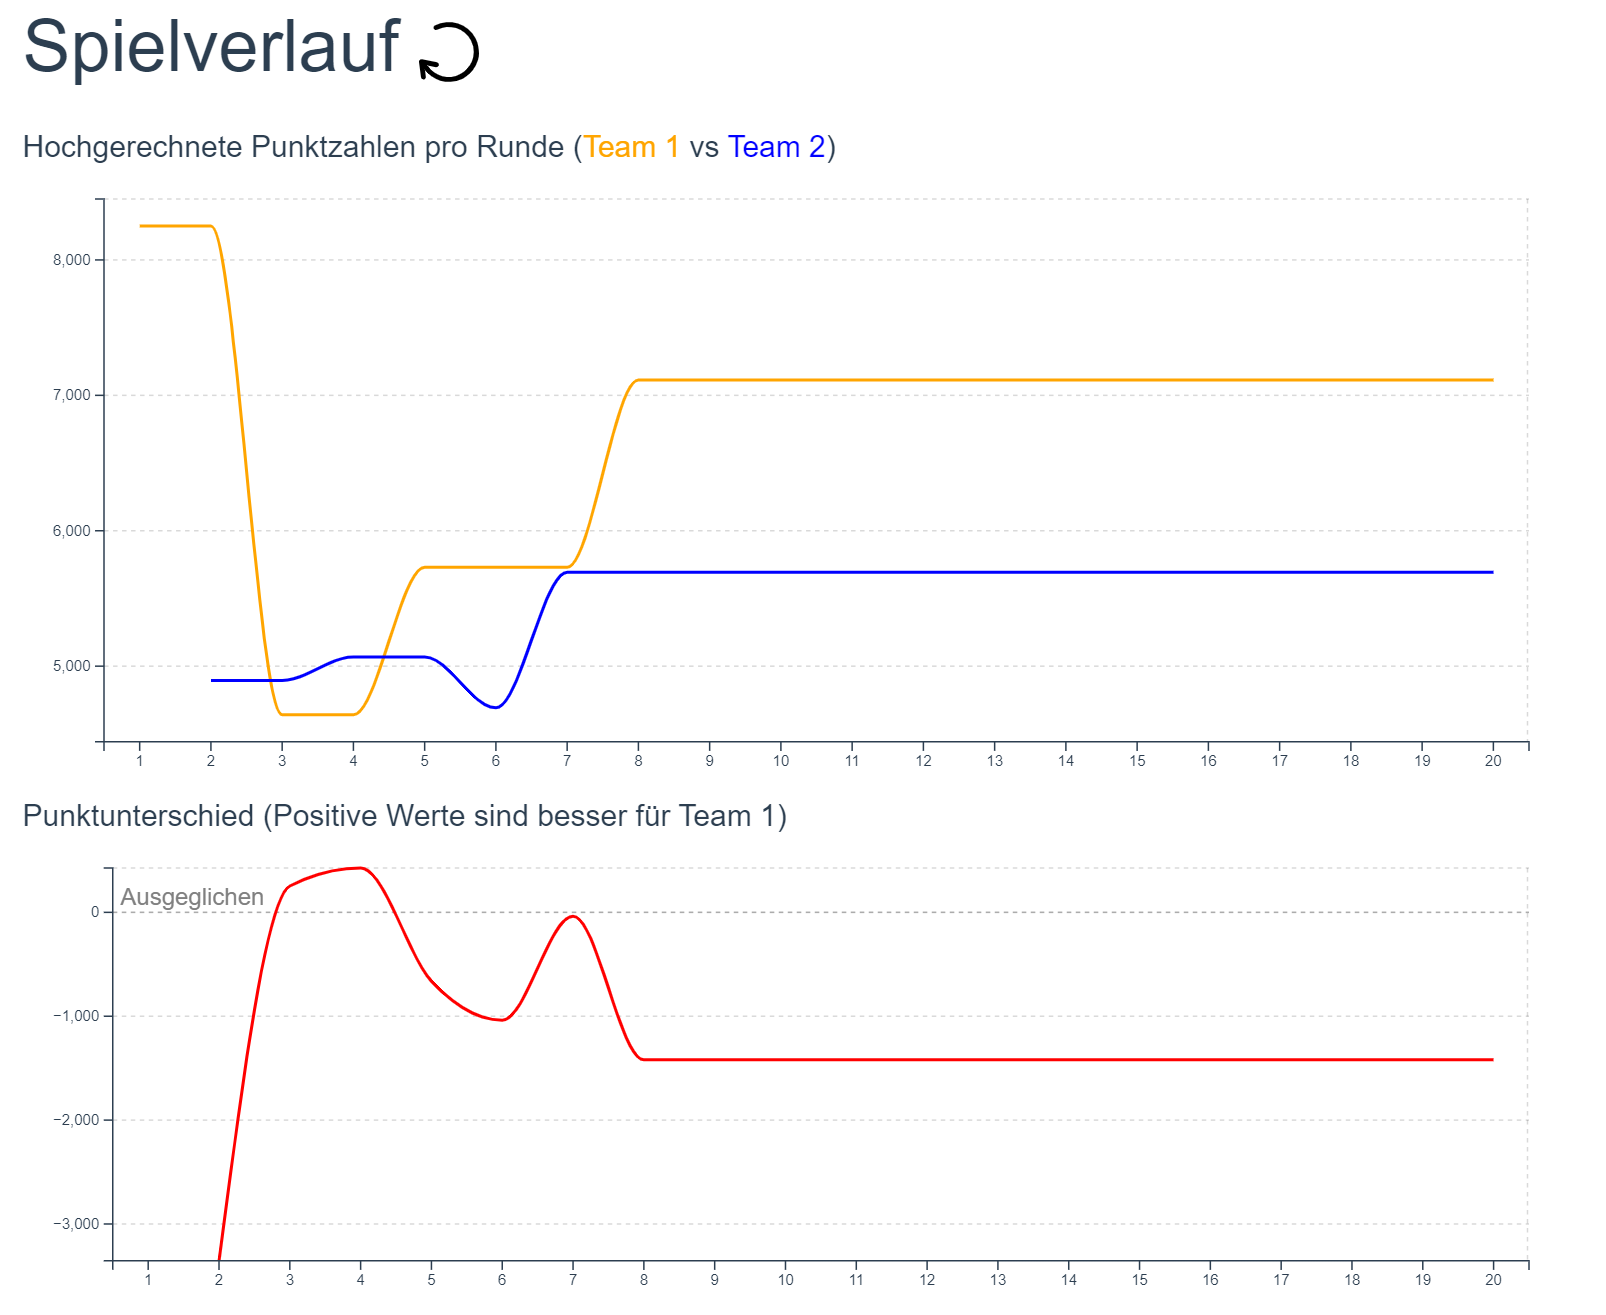
\includegraphics[width=0.9\textwidth]{resources/screenshots/statistics}

\section*{Profile}
If you register to JassTracker instead of playing as a guest, you will never lose access to your games. On top of that you gain access to your individual statistics, to show you just how good you are at the game. You can also set your display name, which will be filled in by default when creating a new game. It can still be changed on a per game basis, so if you find yourself playing Jass with shady figures who should not know your true identity, we've got your back.
